% Options for packages loaded elsewhere
\PassOptionsToPackage{unicode}{hyperref}
\PassOptionsToPackage{hyphens}{url}
%
\documentclass[
  12pt,
]{article}
\usepackage{lmodern}
\usepackage{amssymb,amsmath}
\usepackage{ifxetex,ifluatex}
\ifnum 0\ifxetex 1\fi\ifluatex 1\fi=0 % if pdftex
  \usepackage[T1]{fontenc}
  \usepackage[utf8]{inputenc}
  \usepackage{textcomp} % provide euro and other symbols
\else % if luatex or xetex
  \usepackage{unicode-math}
  \defaultfontfeatures{Scale=MatchLowercase}
  \defaultfontfeatures[\rmfamily]{Ligatures=TeX,Scale=1}
  \setmainfont[]{Times New Roman}
\fi
% Use upquote if available, for straight quotes in verbatim environments
\IfFileExists{upquote.sty}{\usepackage{upquote}}{}
\IfFileExists{microtype.sty}{% use microtype if available
  \usepackage[]{microtype}
  \UseMicrotypeSet[protrusion]{basicmath} % disable protrusion for tt fonts
}{}
\usepackage{xcolor}
\IfFileExists{xurl.sty}{\usepackage{xurl}}{} % add URL line breaks if available
\IfFileExists{bookmark.sty}{\usepackage{bookmark}}{\usepackage{hyperref}}
\hypersetup{
  pdftitle={Geographic and temporal trends in cadmium and lead concentrations in Mytilus edulis (blue mussel) along the Atlantic coast of Europe},
  pdfauthor={Sena McCrory},
  hidelinks,
  pdfcreator={LaTeX via pandoc}}
\urlstyle{same} % disable monospaced font for URLs
\usepackage[margin=2.54cm]{geometry}
\usepackage{longtable,booktabs}
% Correct order of tables after \paragraph or \subparagraph
\usepackage{etoolbox}
\makeatletter
\patchcmd\longtable{\par}{\if@noskipsec\mbox{}\fi\par}{}{}
\makeatother
% Allow footnotes in longtable head/foot
\IfFileExists{footnotehyper.sty}{\usepackage{footnotehyper}}{\usepackage{footnote}}
\makesavenoteenv{longtable}
\usepackage{graphicx,grffile}
\makeatletter
\def\maxwidth{\ifdim\Gin@nat@width>\linewidth\linewidth\else\Gin@nat@width\fi}
\def\maxheight{\ifdim\Gin@nat@height>\textheight\textheight\else\Gin@nat@height\fi}
\makeatother
% Scale images if necessary, so that they will not overflow the page
% margins by default, and it is still possible to overwrite the defaults
% using explicit options in \includegraphics[width, height, ...]{}
\setkeys{Gin}{width=\maxwidth,height=\maxheight,keepaspectratio}
% Set default figure placement to htbp
\makeatletter
\def\fps@figure{htbp}
\makeatother
\setlength{\emergencystretch}{3em} % prevent overfull lines
\providecommand{\tightlist}{%
  \setlength{\itemsep}{0pt}\setlength{\parskip}{0pt}}
\setcounter{secnumdepth}{5}

\title{Geographic and temporal trends in cadmium and lead concentrations in
\emph{Mytilus edulis} (blue mussel) along the Atlantic coast of Europe}
\usepackage{etoolbox}
\makeatletter
\providecommand{\subtitle}[1]{% add subtitle to \maketitle
  \apptocmd{\@title}{\par {\large #1 \par}}{}{}
}
\makeatother
\subtitle{\url{https://github.com/slm119/ENV872_FinalProject}}
\author{Sena McCrory}
\date{}

\begin{document}
\maketitle

\newpage
\tableofcontents 
\newpage
\listoftables

\listoffigures 
\newpage

\hypertarget{rationale-and-research-questions}{%
\section{Rationale and Research
Questions}\label{rationale-and-research-questions}}

Heavy metal pollution is a global environmental and human health concern
(Tchounwou et al., 2012; WHO\textbar Cadmium n.d.; WHO\textbar Lead,
n.d.)). Increasingly, research indicates that there may be no ``safe''
level of heavy metal exposure for humans, and so reducing levels of
these neurotoxic, carcinogenic metals is a continuing battle for global
human health. Heavy metals are also toxic to other organisms and have
been associated with significant decreases biodiversity in natural
systems (Johnston and Roberts, 2009). Cadmium and lead are two heavy
metals which are naturally occurring in the environment but
concentrations have increased due to human activities including fossil
fuel combustion, industrial manufacturing, mining activities, and others
(Tchounwou et al., 2012). Therefore, monitoring the spatial and temporal
distribution of these heavy metal pollutants is essential for
identifying pollution hot spots, avoiding the consumption of
contaminated foods (like marine mussels), and assessing the rate of
athropogenic heavy metal loading in natural systems.

\emph{Mytilus edulis} (blue mussel) are marine bivalves which are
capable of bioaccumulating heavy metals in their soft tissues. These
organisms have been used for decades as a bioindicator for heavy metal
pollution in marine environments (Phillips, 1977). \emph{Mytilus edulis}
are also harvested and farmed commercially for human consumption, and so
monitoring heavy metals in their tissues is also important for managing
potential human health risks. The International Council for the
Exploration of the Sea (ICES) maintains an extensive database of
contaminants in marine biota which includes sampling data for
\emph{Mytilus edulis} from several long-term monitoring programs
throughout Atlantic Europe dating back to 1979. Median concentrations of
cadmium and lead have decreased noticeable between 1979 and 1991 likely
due to environmental regulations put in place during that time such as
the banned use of tetraethyl leaded gasoline (Tchounwou et al., 2012);
however, this decrease has slowed noticeably in recent decades (Fig 3).

For this analysis, I explored two questions concerning cadmium and lead
concentrations in \emph{Mytilus edulis} using the ICES monitoring data
from 1990 to 2018.

\begin{enumerate}
\def\labelenumi{\arabic{enumi}.}
\tightlist
\item
  How have concentrations of cadmium and lead in \emph{Mytilus edulis}
  changed overall in the study region since the 1990s?
\item
  Do cadmium and lead concentrations in \emph{Mytilus edulis} differ by
  country?
\end{enumerate}

\newpage

\hypertarget{dataset-information}{%
\section{Dataset Information}\label{dataset-information}}

The global coastline data used in the study area map is publicly
available through the National Oceanographic and Atmospheric
Administration's (NOAA) National Center for Environmental Information
(NCEI) online data portal located here:
\url{https://www.ngdc.noaa.gov/mgg/shorelines/}. The L1 resolution files
were used from the Global Self-consistent Hierarchical High-resolution
Geography (GSHHG) dataset. Geographic reference system is WGS84 (decimal
degrees).

Data for cadmium and lead concentrations in \emph{Mytilus edulis} were
downloaded from the International Council for the Exploration of the Sea
(ICES) DOME database on Feb 26, 2020 (available here:
\url{http://dome.ices.dk/views/ContaminantsBiota.aspx}). This data
portal holds a collection of marine related monitoring data sourced from
several regional European monitoring groups including ICES, OSPAR,
HELCOM, AMAP, and Expert Groups. Data for all metal and metalloid
concentrations in biota were downloaded and then filtered to include
only \emph{Mytilus edulis} species and the specific heavy metals of
interest for this study. The sampling data for \emph{Mytilus edulis} was
restricted to include only concentrations reported for the ``whole soft
body'' of the bivalve and expressed in mass of metal per mass of the
organism wet weight. There was no information provided to allow a
conversion from dry weight to wet weight concentrations, and so dry
weight records (a small minority of the data) were excluded from the
analysis. Additionally, records flagged as having ``suspect'' data
quality were excluded from the data set. Dataset variables are described
in Table 1 below.

\newpage

\begin{longtable}[]{@{}llll@{}}
\caption{Variable descriptions and statistics for ICES DOME monitoring
data}\tabularnewline
\toprule
\begin{minipage}[b]{0.15\columnwidth}\raggedright
Variable name\strut
\end{minipage} & \begin{minipage}[b]{0.22\columnwidth}\raggedright
Description\strut
\end{minipage} & \begin{minipage}[b]{0.25\columnwidth}\raggedright
Statistics for Cd\strut
\end{minipage} & \begin{minipage}[b]{0.25\columnwidth}\raggedright
Statistics for Pb\strut
\end{minipage}\tabularnewline
\midrule
\endfirsthead
\toprule
\begin{minipage}[b]{0.15\columnwidth}\raggedright
Variable name\strut
\end{minipage} & \begin{minipage}[b]{0.22\columnwidth}\raggedright
Description\strut
\end{minipage} & \begin{minipage}[b]{0.25\columnwidth}\raggedright
Statistics for Cd\strut
\end{minipage} & \begin{minipage}[b]{0.25\columnwidth}\raggedright
Statistics for Pb\strut
\end{minipage}\tabularnewline
\midrule
\endhead
\begin{minipage}[t]{0.15\columnwidth}\raggedright
PARAM\strut
\end{minipage} & \begin{minipage}[t]{0.22\columnwidth}\raggedright
Parameter\strut
\end{minipage} & \begin{minipage}[t]{0.25\columnwidth}\raggedright
``Cd'' -- cadmium (6762 records)\strut
\end{minipage} & \begin{minipage}[t]{0.25\columnwidth}\raggedright
``Pb'' -- lead (6709 records)\strut
\end{minipage}\tabularnewline
\begin{minipage}[t]{0.15\columnwidth}\raggedright
MYEAR\strut
\end{minipage} & \begin{minipage}[t]{0.22\columnwidth}\raggedright
Monitoring year (may differ from the sampling year, NOT used in temporal
trend analysis)\strut
\end{minipage} & \begin{minipage}[t]{0.25\columnwidth}\raggedright
1990 - 2018\strut
\end{minipage} & \begin{minipage}[t]{0.25\columnwidth}\raggedright
1990 - 2018\strut
\end{minipage}\tabularnewline
\begin{minipage}[t]{0.15\columnwidth}\raggedright
DATE\strut
\end{minipage} & \begin{minipage}[t]{0.22\columnwidth}\raggedright
Sample date\strut
\end{minipage} & \begin{minipage}[t]{0.25\columnwidth}\raggedright
February 6, 1990 to Feb 27, 2019\strut
\end{minipage} & \begin{minipage}[t]{0.25\columnwidth}\raggedright
February 6, 1990 to Feb 27, 2019\strut
\end{minipage}\tabularnewline
\begin{minipage}[t]{0.15\columnwidth}\raggedright
Latitude and Longitude\strut
\end{minipage} & \begin{minipage}[t]{0.22\columnwidth}\raggedright
units: decimal degrees\strut
\end{minipage} & \begin{minipage}[t]{0.25\columnwidth}\raggedright
\strut
\end{minipage} & \begin{minipage}[t]{0.25\columnwidth}\raggedright
\strut
\end{minipage}\tabularnewline
\begin{minipage}[t]{0.15\columnwidth}\raggedright
Country\strut
\end{minipage} & \begin{minipage}[t]{0.22\columnwidth}\raggedright
Country where measurement was reported\strut
\end{minipage} & \begin{minipage}[t]{0.25\columnwidth}\raggedright
\strut
\end{minipage} & \begin{minipage}[t]{0.25\columnwidth}\raggedright
\strut
\end{minipage}\tabularnewline
\begin{minipage}[t]{0.15\columnwidth}\raggedright
Value.mgperkg\strut
\end{minipage} & \begin{minipage}[t]{0.22\columnwidth}\raggedright
Concentration of contaminant in subsample. Units: mg metal/kg organism
mass (wet weight of whole soft body).\strut
\end{minipage} & \begin{minipage}[t]{0.25\columnwidth}\raggedright
range DL -- 38.9; median 0.18; mean 0.32\strut
\end{minipage} & \begin{minipage}[t]{0.25\columnwidth}\raggedright
range DL - 98.01; median 0.28; mean 0.01\strut
\end{minipage}\tabularnewline
\begin{minipage}[t]{0.15\columnwidth}\raggedright
NOINP\strut
\end{minipage} & \begin{minipage}[t]{0.22\columnwidth}\raggedright
Number of individuals included in the subsample\strut
\end{minipage} & \begin{minipage}[t]{0.25\columnwidth}\raggedright
range 1-703\strut
\end{minipage} & \begin{minipage}[t]{0.25\columnwidth}\raggedright
range 1-703\strut
\end{minipage}\tabularnewline
\begin{minipage}[t]{0.15\columnwidth}\raggedright
DETLI.mgperkg\strut
\end{minipage} & \begin{minipage}[t]{0.22\columnwidth}\raggedright
Reported detection limit of measurement equipment, units in mg/kg\strut
\end{minipage} & \begin{minipage}[t]{0.25\columnwidth}\raggedright
range 0.000007 to 1; 1792 unreported\strut
\end{minipage} & \begin{minipage}[t]{0.25\columnwidth}\raggedright
range 0.0001 - 0.6; 1736 unreported\strut
\end{minipage}\tabularnewline
\begin{minipage}[t]{0.15\columnwidth}\raggedright
QFLAG\strut
\end{minipage} & \begin{minipage}[t]{0.22\columnwidth}\raggedright
Quality flag (see DOME metadata for full description of codes)\strut
\end{minipage} & \begin{minipage}[t]{0.25\columnwidth}\raggedright
24 \textless; 1 D; 2 Q; 6735 NA\strut
\end{minipage} & \begin{minipage}[t]{0.25\columnwidth}\raggedright
69 \textless; 0 D; 5 Q; 6635 NA\strut
\end{minipage}\tabularnewline
\bottomrule
\end{longtable}

\newpage

\hypertarget{exploratory-analysis}{%
\section{Exploratory Analysis}\label{exploratory-analysis}}

\hypertarget{geographic-distribution-of-monitoring-data}{%
\subsection{Geographic distribution of monitoring
data}\label{geographic-distribution-of-monitoring-data}}

\begin{figure}
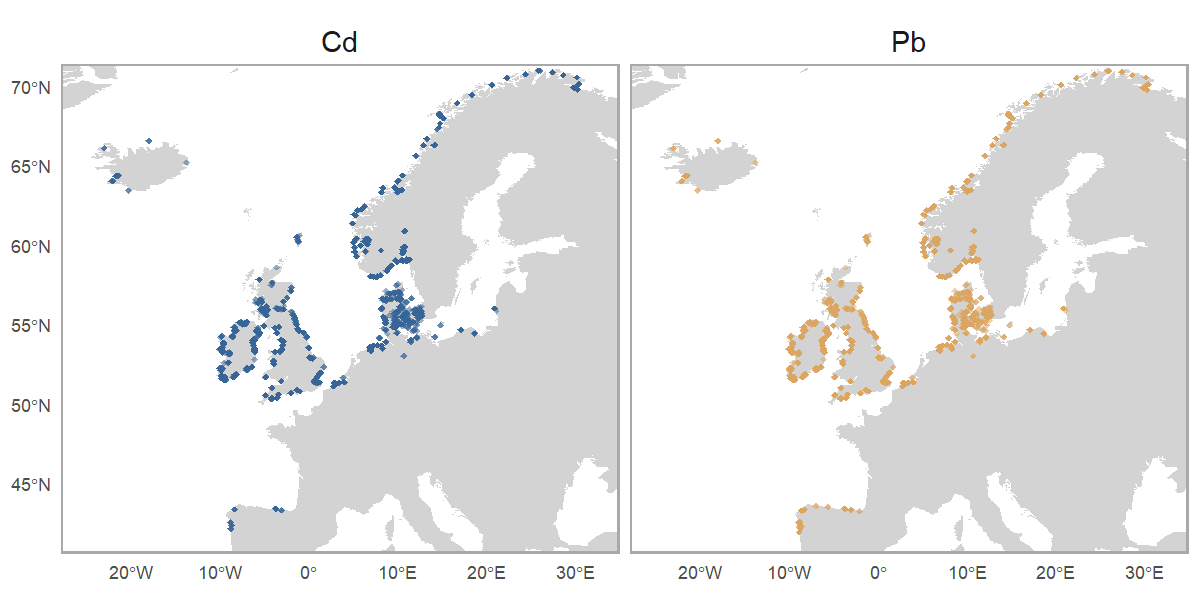
\includegraphics[width=0.92\linewidth]{C:/Users/senam/Box Sync/My Documents/MEM classes/Duke Spring 2020/DataAnalytics/ENV872_FinalProject/Output/StudyRegionMap2} \caption{Monitoring locations of ICES DOME database records for cadmium and lead concentrations *Mytilus edulis* from 1990 to 2018}\label{fig:unnamed-chunk-1}
\end{figure}

Sample locations are highly clustered near European Atlantic and North
Sea shorelines (Fig 1). Geographic spread of the sample sites are
similar for cadmium and lead (Fig 1). The total number of samples during
the study period varied significantly by country. For both metals,
Norway accounted for about 43 percent of all the records (Fig 2). The
top four countries with the most records (Norway, UK, Ireland, and
Denmark) accounted for 90.9 percent of all records for cadmium and 89.3
percent of all records for lead (Fig 2). In general, sample numbers were
similar between cadmium and lead because in many cases each
\emph{Mytilus edulis} sample was tested for both types of metals except
Spain did not include many records for cadmium. Sampling records were
sparse for coastlines in the Baltic Sea. Other coastal European nations
including France, Sweden, Finland, Estonia, Lithuania, and Poland did
not have any sampling records in this database.

\begin{figure}
\centering
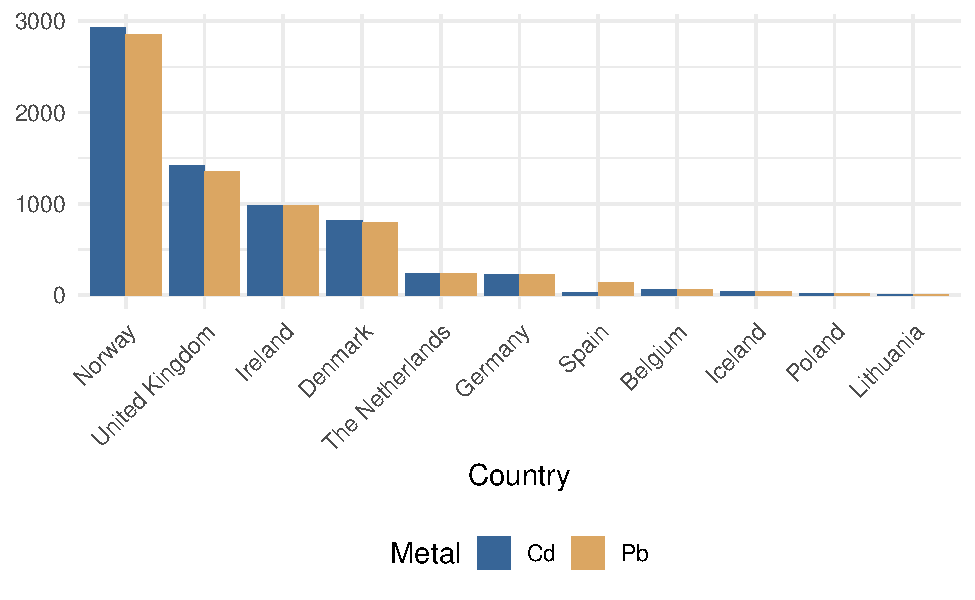
\includegraphics{McCrory_ENV972_Project_files/figure-latex/unnamed-chunk-2-1.pdf}
\caption{Number of \emph{Mytilus edulis} cadmium and lead monitoring
records by country between 1990 and 2019.}
\end{figure}

\hypertarget{temporal-distribution-of-monitoring-data}{%
\subsection{Temporal distribution of monitoring
data}\label{temporal-distribution-of-monitoring-data}}

Yearly median concentrations in \emph{Mytilus edulis} for both cadmium
and lead concentrations show a noticeable decrease between 1979 to about
1990 (Fig 3). After 1990, however, the temporal trend is less obvious; a
monthly time series analysis was used to determine whether a there is a
monotonic trend after 1990. For both metals, April, May, June, and July
were most likely to have missing sample data during the study period and
September through November were the most compete months with at least
one record for every year in the dataset (Table 2).

\begin{figure}
\centering
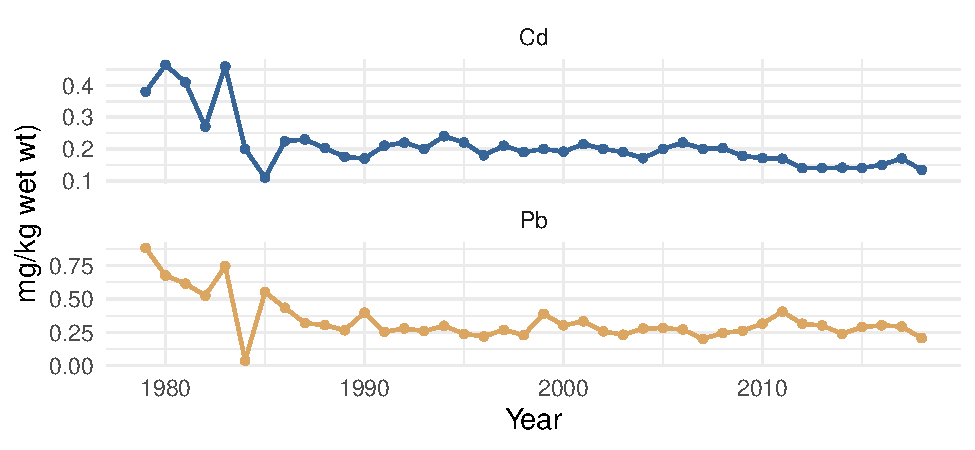
\includegraphics{McCrory_ENV972_Project_files/figure-latex/unnamed-chunk-3-1.pdf}
\caption{Yearly median concentrations of cadmium and lead in
\emph{Mytilus edulis} ICES monitoring data from 1979 to 2018. Notice the
stark decrease from 1979 to the late 1980s and the leveling off after
1990.}
\end{figure}

\begin{longtable}[]{@{}lll@{}}
\caption{Sampling percentage for each month during the analysis study
period from Feb 1990 to Jan 2019. September, October, and November were
the only months with sampling data for all years.}\tabularnewline
\toprule
Month & Cd & Pb\tabularnewline
\midrule
\endfirsthead
\toprule
Month & Cd & Pb\tabularnewline
\midrule
\endhead
January & 55\% & 59\%\tabularnewline
February & 76\% & 72\%\tabularnewline
March & 79\% & 79\%\tabularnewline
April & 45\% & 45\%\tabularnewline
May & 28\% & 28\%\tabularnewline
June & 31\% & 31\%\tabularnewline
July & 31\% & 28\%\tabularnewline
August & 76\% & 76\%\tabularnewline
September & 100\% & 100\%\tabularnewline
October & 100\% & 100\%\tabularnewline
November & 100\% & 100\%\tabularnewline
December & 76\% & 76\%\tabularnewline
\bottomrule
\end{longtable}

\hypertarget{distribution-of-cadmium-and-lead-concentrations}{%
\subsection{Distribution of cadmium and lead
concentrations}\label{distribution-of-cadmium-and-lead-concentrations}}

Concentrations for cadmium ranged from below the instrument detection
limit to 98.1 mg/kg with a median of 0.28 mg/kg and mean of 0.81 mg/kg.
Lead concentrations ranged from below the detection limit to 38.9 mg/kg
with a median of 0.18 mg/kg and mean of 0.32 mg/kg. Both metals
exhibited a strong positive skew and so are displayed on a log scale in
most figures. Detection limits for measurement instruments ranged
substantially for both metal samples (Table 1), and many samples
concentrations were within the range of detection limits for other
samples (Fig 5). This results in considerable left censoring of the data
which can affect interpretation of statistical analyses.

\begin{figure}
\centering
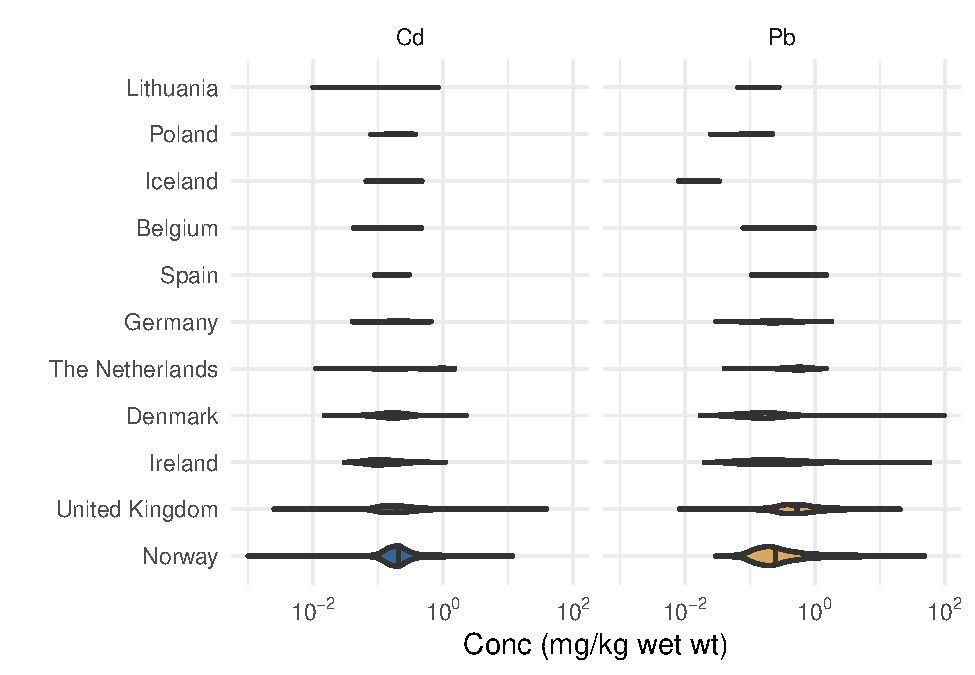
\includegraphics{McCrory_ENV972_Project_files/figure-latex/unnamed-chunk-5-1.pdf}
\caption{Distribution of cadmium and lead concentrations in
\emph{Mytilus edulis} sample records from 1990 to 2019.}
\end{figure}

\begin{figure}
\centering
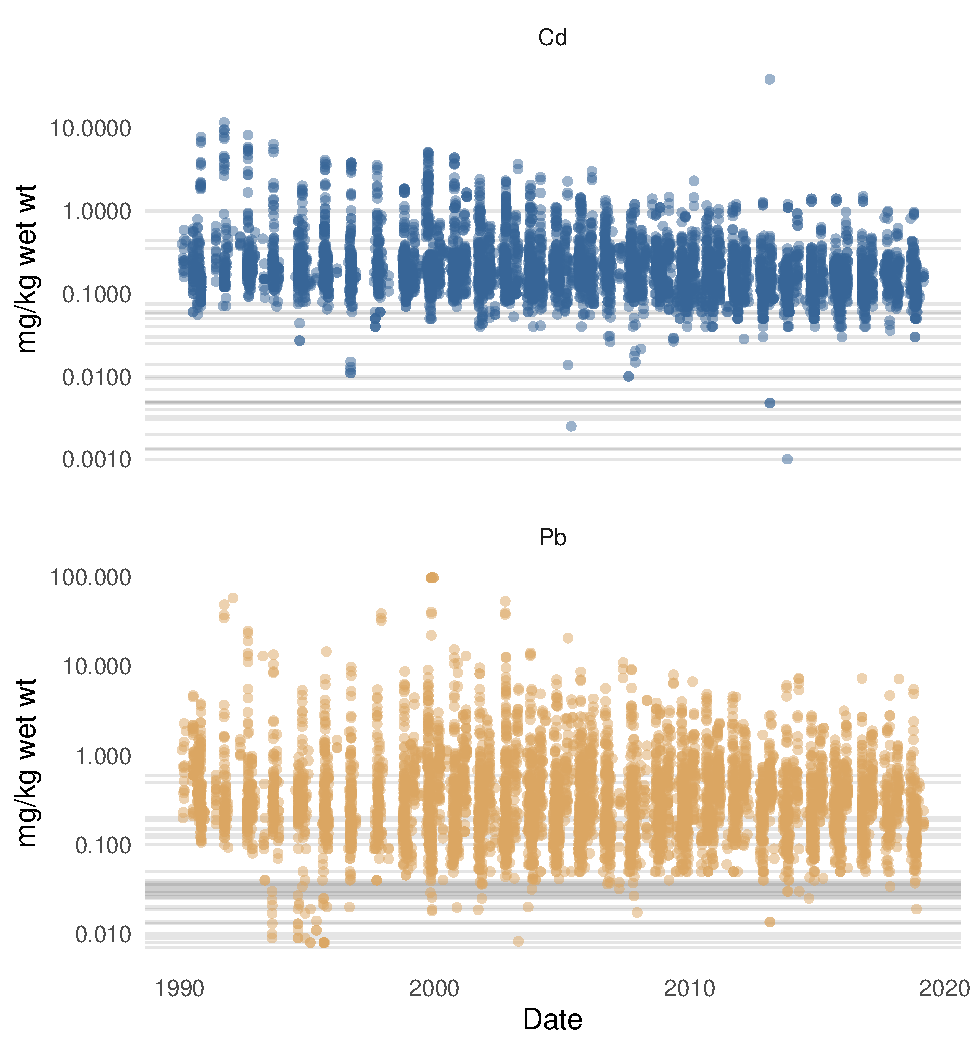
\includegraphics{McCrory_ENV972_Project_files/figure-latex/unnamed-chunk-6-1.pdf}
\caption{Concentrations of cadmium and lead in ICES \emph{Mytilus
edulis} monitoring samples for all sample dates from Feb 1990 to Jan
2019. Grey lines indicate the various instrument detection limits
reported in each the data set.}
\end{figure}

\newpage

\hypertarget{analysis}{%
\section{Analysis}\label{analysis}}

\hypertarget{question-1-how-have-cadmium-and-lead-concentrations-in-mytilus-edulis-changed-over-time}{%
\subsection{\texorpdfstring{Question 1: How have cadmium and lead
concentrations in \emph{Mytilus edulis} changed over
time?}{Question 1: How have cadmium and lead concentrations in Mytilus edulis changed over time?}}\label{question-1-how-have-cadmium-and-lead-concentrations-in-mytilus-edulis-changed-over-time}}

Data for lead and cadmium concentrations were aggregated based on the
monthly median for each month between February 1990 to January 2019.
Months with no sample data were interpolated using a linear
interpolation (Fig 6).

Cadmium concentrations in \emph{Mytilus edulis} have decreased
significantly over the study period by an estimated 0.002 mg/kg from
1990 to 2019 (Seasonal Mann-Kendall; S = -1044; p \textless0.0001;
Seasonal Sen's Slope). Cadmium concentrations also exhibited some
seasonal variability; higher decreasing trends were seen in November,
December, and January as compared to other months of the year (Seasonal
Sen;s Slope, p \textless{} 0.05). Lead showed no significant monotonic
trend over the study period (Seasonal Mann-Kendall; S = -284; p =
0.125).

\begin{figure}
\centering
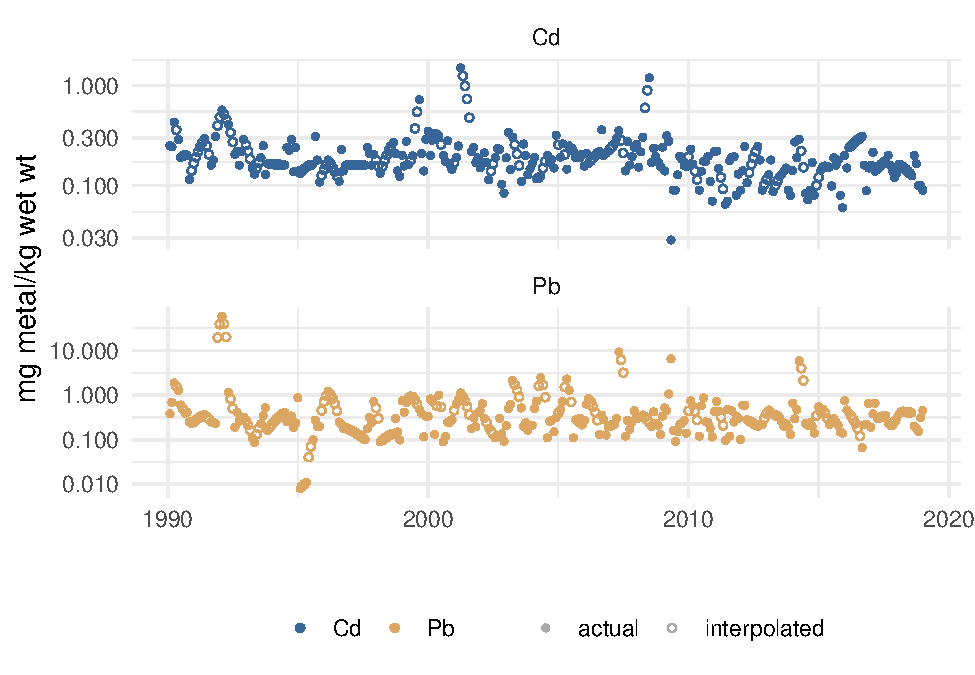
\includegraphics{McCrory_ENV972_Project_files/figure-latex/unnamed-chunk-7-1.pdf}
\caption{Monthly median cadmium and lead concentrations in \emph{Mytilus
edulis} from 1990 to 2018. Points symbolized with open circles are
linearly interpolated.}
\end{figure}

\newpage

\hypertarget{question-2-do-cadmium-and-lead-concentrations-in-mytilus-edulis-differ-by-country}{%
\subsection{\texorpdfstring{Question 2: Do cadmium and lead
concentrations in \emph{Mytilus edulis} differ by
country?}{Question 2: Do cadmium and lead concentrations in Mytilus edulis differ by country?}}\label{question-2-do-cadmium-and-lead-concentrations-in-mytilus-edulis-differ-by-country}}

Comparison of concentrations between countries was restricted to only
countries with more than 100 records over the study period. Due to the
non-normal, heterogenous variance, and unequal sample size of the data,
a non-parametric group-wise comparison was used to compare concentration
distributions by country.

Analyses for cadmium revealed that concentration distributions differed
significantly between all countries except Germany and the UK which were
statistically similar (Fig 7; Kruskal-Wallis Rank Sum Test, chi-squared
= 897.8, df = 5, p \textless{} 0.0001; Dunn's Test with
Benjamin-Hochberg (1995) adjustment, p \textless{} 0.05 for all
comparisons except Germany and UK). The Netherlands had the highest
distribution of cadmium concentrations with a median of 0.41 mg/kg (see
Table 3).

\begin{figure}
\centering
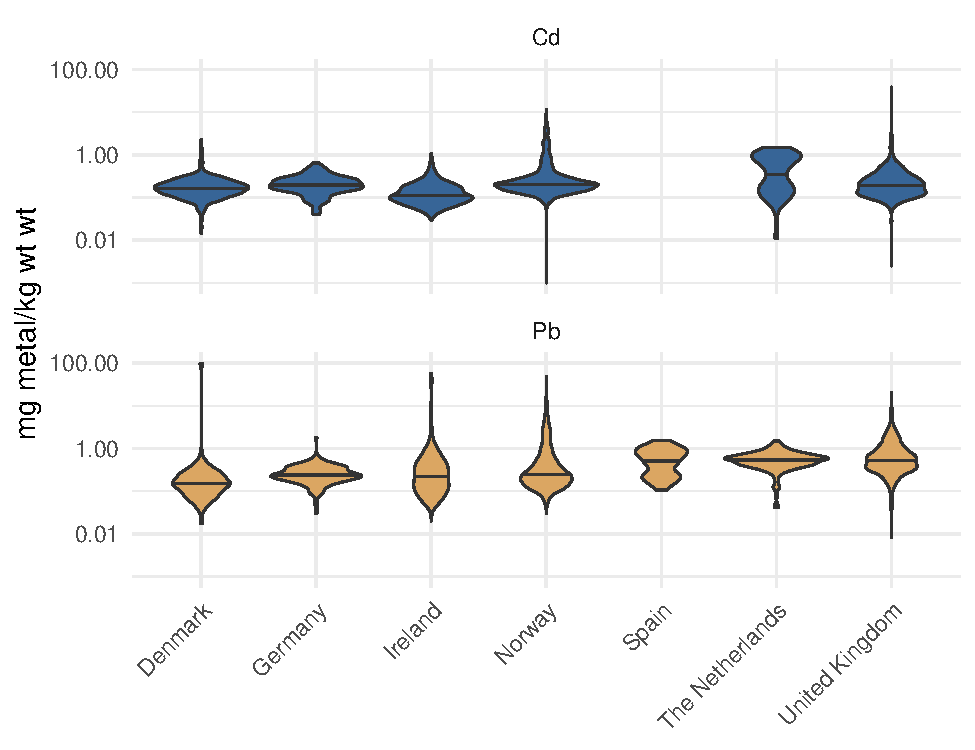
\includegraphics{McCrory_ENV972_Project_files/figure-latex/unnamed-chunk-8-1.pdf}
\caption{Distribution of cadmium and lead concentrations in
\emph{Mytilus edulis} for countries with more than 100 samples between
1990 and 2018.}
\end{figure}

Lead concentration distributions between countries also differed
significantly by country (Fig 7; Kruskal-Wallis Rank Sum Test,
chi-squared = 1302.8, df = 6, p \textless{} 0.0001; Dunn's Test with
Benjamin-Hochberg (1995) adjustment, p \textless{} 0.05). The
Netherlands, Spain, and UK had the highest distribution of lead
concentrations and were statistically similar to each other. Next
highest lead concentrations were in Norway, then Germany and Ireland
(not significantly different from each other, but were different from
all other groups), and then the lowest lead concentrations were in
Denmark (Dunn's Test, alpha = 0.05).

\begin{longtable}[]{@{}lll@{}}
\caption{Median concentrations of cadmium and lead in \emph{Mytilus
edulis} by country during the study period from 1990 --
2019.}\tabularnewline
\toprule
Country & Median Cd conc (mg/kg) & Median Pb conc (mg/kg)\tabularnewline
\midrule
\endfirsthead
\toprule
Country & Median Cd conc (mg/kg) & Median Pb conc (mg/kg)\tabularnewline
\midrule
\endhead
The Netherlands & 0.41 & 0.55\tabularnewline
Spain & - & 0.49\tabularnewline
Norway & 0.21 & 0.25\tabularnewline
Germany & 0.20 & 0.24\tabularnewline
United Kingdom & 0.19 & 0.54\tabularnewline
Denmark & 0.16 & 0.15\tabularnewline
Ireland & 0.11 & 0.22\tabularnewline
\bottomrule
\end{longtable}

\newpage

\hypertarget{summary-and-conclusions}{%
\section{Summary and Conclusions}\label{summary-and-conclusions}}

Long term monitoring efforts for \emph{Mytilus edulis} allow researchers
to gauge our progress in reducing heavy metal contaminants in marine
ecosystems. However, it is important to consider the limitations of
using data which was collected over many years and from numerous testing
programs. One of the limitations in this investigation is the wide array
of sampling methods, analysis methods, and varying instrument detection
limits used in the data collection process. Some of the analytical
equipment used for monitoring efforts were not able to detect metal
concentrations below 0.6 or even 1 mg/kg, while other testing facilities
recorded metal concentrations well below these detection limits at 0.01
mg/kg or less. A high number of left-censored records could lead to an
under or over-estimate of the true trends in metal concentrations over
time. Therefore, it would beneficial to update metal testing procedures
to use more sensitive tests that are able to precisely measure
environmentally-relevant concentrations of cadmium and lead in marine
organisms.

This analysis of heavy metals trends in the European Atlantic coastal
region suggest that, as a whole, concentrations of cadmium have
decreased by a small but significantly amount since 1990. Current median
concentration of cadmium in \emph{Mytilus eduils} remains well below the
current United Nations Food and Agricultural Organization's (UN FAO)
suggested maximum level of 2 mg/kg in marine bivalves for human
consumption, but efforts are still needed to reduce cadmium
concentrations to background levels (FAO, 2019). Lead concentrations,
however, were not found to have decreased significantly over the same
study period, and several countries were found to have much higher lead
loads than others.

Cadmium and lead concentrations in \emph{Mytilus edulis} were shown to
vary regionally. The Netherlands was consistently shown to have the
highest concentrations of both heavy metals. Spain and the UK also had
significantly higher levels of lead bioaccumulation in their monitoring
samples than the other countries included in this analysis. These
results suggest that management efforts at the regional or national
level may have direct implications for heavy metal loading in coastal
environments. Future analysis should be done to identify identify major
sources of cadmium and lead and identify effective management and policy
efforts that can help reduce heavy metal releases to coastal
environments.

\newpage

\hypertarget{references}{%
\section{References}\label{references}}

FAO. (2019). Codex Alimentarius: GENERAL STANDARD FOR CONTAMINANTS AND
TOXINS IN FOOD AND FEED. United Nations, Food and Agriculture
Organization, CXS 193-1995.

Johnston, E. L., \& Roberts, D. A. (2009). Contaminants reduce the
richness and evenness of marine communities: A review and meta-analysis.
Environmental Pollution, 157(6), 1745--1752.
\url{https://doi.org/10.1016/j.envpol.2009.02.017}

Phillips, D. J. H. (1977). The use of biological indicator organisms to
monitor trace metal pollution in marine and estuarine environments---A
review. Environmental Pollution (1970), 13(4), 281--317.
\url{https://doi.org/10.1016/0013-9327(77)90047-7}

Tchounwou, P. B., Yedjou, C. G., Patlolla, A. K., \& Sutton, D. J.
(2012). Heavy Metals Toxicity and the Environment. EXS, 101, 133--164.
\url{https://doi.org/10.1007/978-3-7643-8340-4_6}

WHO \textbar{} Cadmium. (n.d.). WHO; World Health Organization.
Retrieved April 20, 2020, from
\url{http://www.who.int/ipcs/assessment/public_health/cadmium/en/}

WHO \textbar{} Lead. (n.d.). WHO; World Health Organization. Retrieved
April 17, 2020, from
\url{http://www.who.int/ipcs/assessment/public_health/lead/en/}

\end{document}
